\documentclass[aspectratio=169]{beamer}

%==============================================================================
% Preamble
%==============================================================================

\usetheme{hogent}
\usecolortheme{hgwhite} % white background, black text

%% common.tex -- Code die in elk .tex-bestand terug komt

%% Packages

\usepackage{graphicx,multicol}
\usepackage{comment,enumerate,hyperref}
\usepackage{amsmath,amsfonts,amssymb}
\usepackage[dutch]{babel}
\usepackage{multirow}
\usepackage{eurosym}
\usepackage{listings}
\usepackage{textcomp}
\usepackage{framed}
\usepackage{wrapfig}
\usepackage{booktabs}
\usepackage{pgfplots}

\pgfplotsset{compat=1.18}
\usetikzlibrary{arrows,shapes,backgrounds,positioning,shadows}

%% Variabelen, elk academiejaar aan te passen
\newcommand{\academicyear}{2023--2024}
\newcommand{\lecturers}{Stijn Lievens}

%% Macro's en commando's die vaak gebruikt worden

% Gauss belcurve
\pgfmathdeclarefunction{gauss}{2}{%
  \pgfmathparse{1/(#2*sqrt(2*pi))*exp(-((x-#1)^2)/(2*#2^2))}%
}
 % Settings and metadata for all slide decks



\usepackage{listings, xcolor}
\lstset{
	tabsize = 4, %% set tab space width
	showstringspaces = false, %% prevent space marking in strings, string is defined as the text that is generally printed directly to the console
	numbers = left, %% display line numbers on the left
	commentstyle = \color{purple}, %% set comment color
	keywordstyle = \color{blue}, %% set keyword color
	stringstyle = \color{red}, %% set string color
	rulecolor = \color{black}, %% set frame color to avoid being affected by text color
	basicstyle = \footnotesize \ttfamily , %% set listing font and size
	breaklines = true, %% enable line breaking
	numberstyle = \tiny,
}


\title{Machine Learning}
\subtitle{Een nieuwe vorm van programmeren}
\author{\lecturers}    % Names of the lecturers - change in common.tex
\date{\academicyear}   % Academic year - change in common.tex

%==============================================================================
% Presentation content
%==============================================================================

\begin{document}

\begin{frame}
  \maketitle
\end{frame}

\begin{frame}
  \frametitle{Inhoud}

  \tableofcontents
\end{frame}

\section{Artifici\"ele Intelligentie}

\begin{frame}
\frametitle{Artifici\"ele Intelligentie}

Waar denk jij aan bij de term Artifici\"ele Intelligentie?

\vspace{1cm}

\pause
\includegraphics[width=0.3\textwidth, height=0.5\textheight]{graphics/chatgpt}
\includegraphics[width=0.3\textwidth,height=0.5\textheight]{graphics/stable-diffusion}
\includegraphics[width=0.3\textwidth,height=0.5\textheight]{graphics/tesla-optimus}

\end{frame}

\begin{frame}
\frametitle{Wat is Artifici\"ele Intelligentie?}
\begin{columns}
	\begin{column}{0.5\textwidth}
		\begin{center}
	\colorbox{yellow}{\Large{\textbf{Artificieel}}}
	\begin{itemize}
		\item Niet op een natuurlijke manier
		\item Kunstmatig
	\end{itemize}
	\end{center}
	\end{column}
	\begin{column}{0.5\textwidth}  %%<--- here
		\begin{center}
			\colorbox{yellow}{\Large{\textbf{Intelligentie}}}
		\end{center}
	\begin{itemize}
		\item Relatief moeilijk te defini\"eren.
		\item Veel verschillende definities.
		\item Filosofen vs.\ psychologen
	\end{itemize}
	\end{column}
\end{columns}
\end{frame}

\begin{frame}
\frametitle{Gangbare praktische definitie}

\begin{block}{Definitie AI-systeem}
Een AI-systeem is een {\emph{computersysteem}} dat {\emph{zelfstandig leert}}, {\emph{beslissingen neemt}}
en {\emph{deze uitvoert}}.
\end{block}

Bron: boek \lq\lq Mens vs.\ Machine\rq\rq\ door Geertrui Mieke de Ketelaere.	
\end{frame}

\begin{frame}
\frametitle{Onderdelen van AI}
\begin{center}
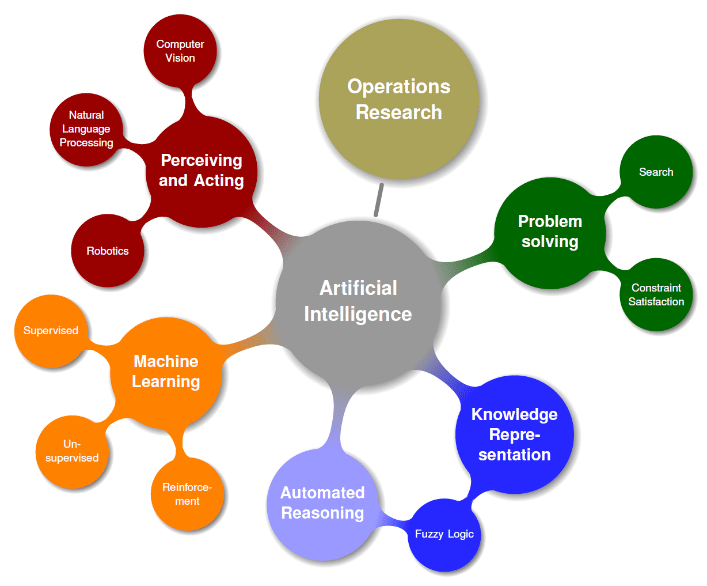
\includegraphics[width=0.6\textwidth]{graphics/areas-of-ai}
\end{center}
\tiny {Bron: \url{https://www.researchgate.net/figure/Different-Areas-Under-Artificial-Intelligence-2_fig1_343079524}}
\end{frame}

\section{Traditioneel Programmeren?}

\begin{frame}
\frametitle{Traditioneel Programmeren?}

Schrijven van een \textbf{spam filter}.

\begin{itemize}
\item Hoe ziet spam er typisch uit?
\pause
\begin{itemize}
	\item \lq\lq 4U\rq\rq, \lq\lq free\rq\rq, \lq\lq credit card\rq\rq, VEEL HOOFDLETTERS
\end{itemize}	
\item Schrijf een algoritme om de patronen hierboven te detecteren.
\item Test programma en herhaal stappen 1 en 2.
\end{itemize}

\end{frame}

\begin{frame}[fragile=singleslide]
\frametitle{Mogelijke Code}
\begin{lstlisting}[language = Python , frame = trBL , firstnumber = 1 , escapeinside={(*@}{@*)}]
def is_spam(email):
	if heeft_veel_hoofdletters(email):
		return True
	if aantal_voorkomens(email, "credit card") > 2:
		if header(email) != "Mijn bank":
			return True
	if aantal_spellingsfouten(email) > 10:
		if afzender(email) != "Mijn vriend":
			return True
		else:
			return False
	# Nog heel veel andere regels
	return False
\end{lstlisting}
\end{frame}

\begin{frame}
\frametitle{Problemen met deze Aanpak?}
\pause
\begin{itemize}
\item De lijst met regels wordt snel heel lang en complex; je zal veel pogingen nodig hebben om de lijst op punt te stellen.
\item Wat als de spammers doorkrijgen hoe jouw lijst werkt?
\begin{itemize}
	\item Dan kan je herbeginnen!
\end{itemize}
\end{itemize}
\end{frame}

\section{Machinaal Leren}

\begin{frame}
\frametitle{Wat is Machinaal Leren?}
\begin{block}{Machinaal Leren}
\emph{Machinaal Leren} is de wetenschap (en kunst) om computers te programmeren zodanig dat ze kunnen \emph{leren van data}.
(Hands-on Machine Learning with Scikit-Learn, Keras and Tensorflow door Aur\'elien G\'eron.)
\end{block}

\begin{block}{Machinaal Leren}
	\emph{Machinaal Leren} is het studiegebied dat computers de mogelijkheid geeft om te leren zonder \emph{expliciet} geprogrammeerd te zijn.
	 (Arthur Samuel, 1959)
\end{block}
\end{frame}


\begin{frame}
\frametitle{Toepassingen van ML}
Welke toepassingen van machinaal leren ken jij?
\pause
\begin{itemize}
	\item Spamdetectie
	\item Classificatie van beelden
	\item Fraudedetectie bij creditkaarten
	\item Aanbevelingssystemen (recommendation systems)
	\item Spraakherkenning (bv.\ Siri, Alexa, $\ldots$)
	\item Genereren van teksten, beelden (bv.\ ChatGPT, MidJourney)
	\item $\ldots$
\end{itemize}
\end{frame}

\begin{frame}
\frametitle{Voorbeelden}
\begin{center}
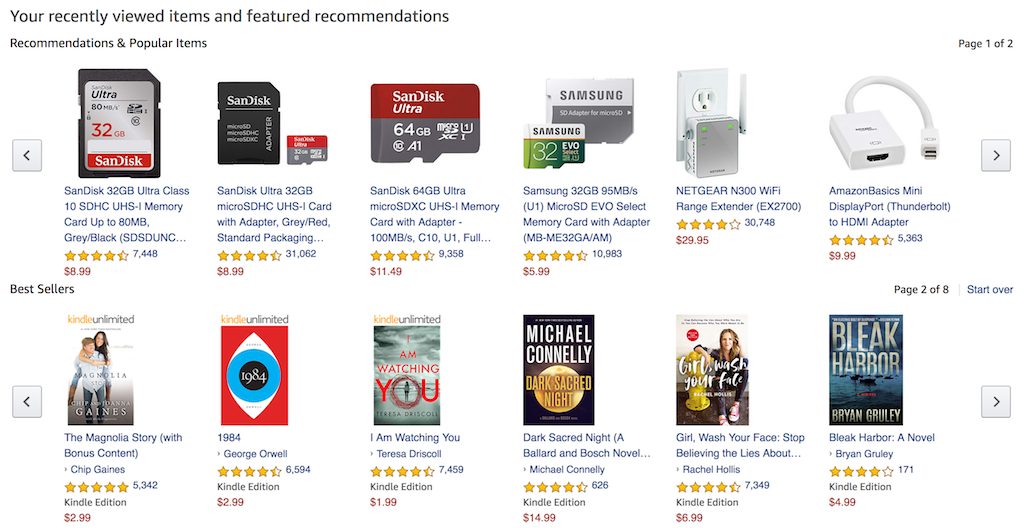
\includegraphics[width=0.4\textwidth]{graphics/amazon-recommendation}
\quad
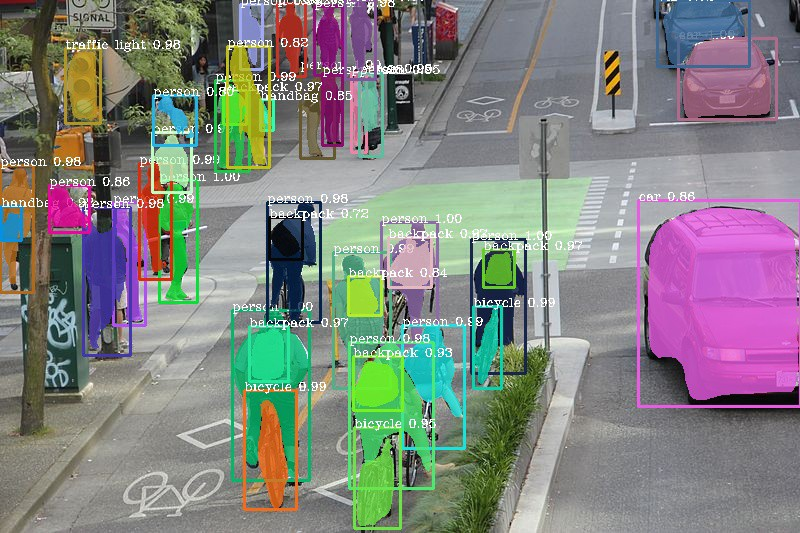
\includegraphics[width=0.4\textwidth]{graphics/beeld-segmentatie}
\end{center}
\tiny{Bronnen: \url{https://emerj.com/ai-sector-overviews/artificial-intelligence-at-amazon/} en  \url{https://towardsdatascience.com/image-segmentation-with-six-lines-0f-code-acb870a462e8}}
\end{frame}

\begin{frame}
\frametitle{Verschillende Soorten ML}

\begin{itemize}
	\item \textbf{Gesuperviseerd} leren. (Eng.\ supervised learning)
	\begin{itemize}
		\item Gegeven veel gelabelde voorbeelden (bv.\ emails met label spam/ham) bepaal het label voor een nieuw voorbeeld.
	\end{itemize}
	\item \textbf{Ongesuperviseerd} leren. (Eng.\ unsupervised learning)	
	\begin{itemize}
		\item Ontdek structuur in ongelabelde data. (bv.\ clustering)
	\end{itemize}
	\item \textbf{Reinforcement} learning.
	\begin{itemize}
		\item Leer een beleid (Eng.\ policy) dat de grootste beloning op lange termijn oplevert.
		Zie bv.\ \url{https://www.youtube.com/watch?v=V1eYniJ0Rnk}
	\end{itemize}
\end{itemize}
\end{frame}

\begin{frame}
\frametitle{Soorten ML}
	\begin{center}
		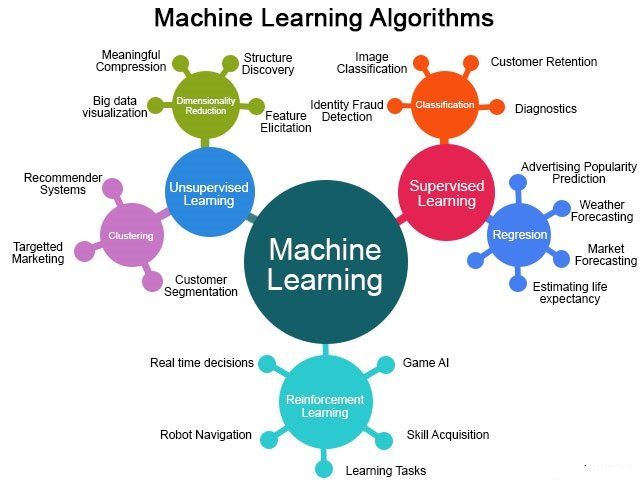
\includegraphics[width=0.6\textwidth]{graphics/soorten-ml}		
	\end{center}
	\tiny{Bron:\url{https://www.researchgate.net/figure/Categorization-of-Machine-Learning-5_fig4_343079524}}
\end{frame}

\section{Lineaire Regressie}


\begin{frame}
\frametitle{Notebook Lineaire Regressie}

Open de Jupyter notebook  \texttt{LineaireRegressie.ipynb} op Google Colab 
(\url{https://colab.research.google.com}).

\vspace{0.5cm}

Deze notebook is beschikbaar op \url{https://github.com/HoGentTIN/ml-workshop-middelbaar}

\end{frame}

\begin{frame}
\frametitle{Lineaire Regressie}

Samenvatting notebook \texttt{LineaireRegressie.ipynb}.

\vspace{0.5cm}

\begin{itemize}
\item Definieer een model met \textbf{parameters}: $a$ en $b$ in dit geval.
\item Definieer een \textbf{kostfunctie} die de kwaliteit van de parameters aangeeft (kleiner is beter).
\item Minimaliseer deze kostfunctie m.b.v.\ \textbf{gradient descent}: dit geeft je dan de beste parameters voor jouw model.
\end{itemize}

\end{frame}

\begin{frame}
\frametitle{Conclusie Lineaire Regressie}

\begin{block}{Conclusie}
	De drie voorgaande stappen:
	\begin{itemize}
		\item Model
		\item Kostfunctie
		\item Optimalisatie m.b.v.\ gradient descent
	\end{itemize}
    zijn de basisstappen voor heel veel modellen van gesuperviseerd leren.
\end{block}

Echter! Nog veel andere technieken nodig om dit praktisch te laten werken op ingewikkelde problemen.

\end{frame}

\section{Neurale Netwerken}


\begin{frame}
	\frametitle{(Binaire) classificatie}
	\begin{itemize}
		\item Bij \textbf{binaire classificatie} tracht men de invoer te classificeren als 1 van 2 mogelijke klassen.
		\item Bv.\ spam of ham, kat of hond, of $\ldots$ \url{https://www.youtube.com/watch?v=tWwCK95X6go}
		\item Bij \textbf{classificatie} zijn er meerdere klassen, bv.\ E-mails worden in verschillende 
		folders geclassificeerd: "Primary", "Social", "Reclame".
	\end{itemize}
\end{frame}

\begin{frame}
\frametitle{Neurale netwerken}

\begin{center}
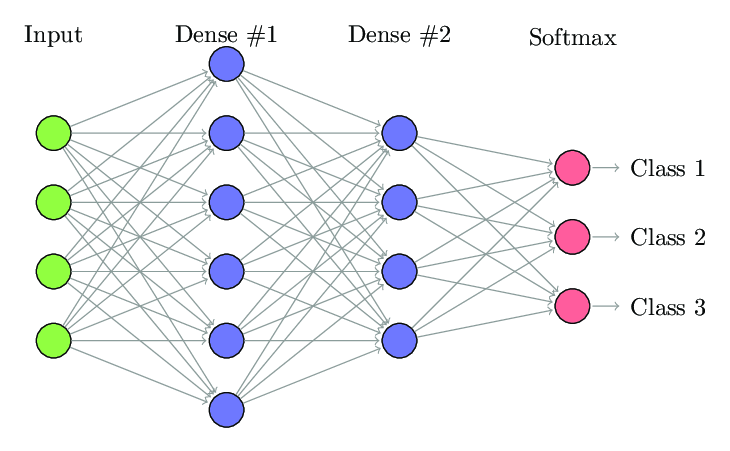
\includegraphics[width=0.8\textwidth]{graphics/fully-connected-neural-network}
\end{center}

\tiny{Bron: \url{https://www.researchgate.net/figure/Example-of-fully-connected-neural-network_fig2_331525817}} 
\end{frame}


\begin{frame}
\frametitle{Neurale netwerken}
\begin{itemize}
\item Een neuraal netwerk bestaat uit een groot aantal \textbf{neuronen}.
\begin{itemize}
	\item Elk neuron doet een \textbf{heel eenvoudige berekening}: nl.\ een gewogen gemiddelde 
	van de invoer gevolgd door een activatiefunctie.
\end{itemize}
\item De uitvoer van een neuron wordt de invoer voor andere neuronen.
\item Neuronen worden typisch georganiseerd in \textbf{lagen}. 
\begin{itemize}
	\item Als er veel lagen zijn: een \lq\lq diep\rq\rq\ neuraal netwerk $\implies$ \lq\lq deep learning\rq\rq.
\end{itemize}
\item De parameters van het model zijn de sterktes van de verbindingen tussen de neuronen.
\begin{itemize}
	\item Deze parameters worden aangepast tijdens het trainen van het neuraal netwerk.
\end{itemize}
\end{itemize}
\end{frame}

\begin{frame}
\frametitle{Tensorflow Playground}
Ga naar \url{https://playground.tensorflow.org/}.

\vspace{0.5cm}

Doe de opdracht die hier beschreven staat: \url{https://developers.google.com/machine-learning/crash-course/introduction-to-neural-networks/playground-exercises}
\end{frame}

\section{Beeldverwerking}

\begin{frame}
\frametitle{Computerafbeeldingen?}


Een computer \lq\lq ziet\rq\rq\ een foto/afbeelding eigenlijk als niets anders dan een raster van getallen.
\begin{itemize}
	\item Getallen zijn vaak gehele getallen tussen 0 en 255.
	\item Voor een zwart/wit foto is er \'e\'en getal per pixel.
	\item Voor een kleurenfoto zijn er drie waarden per pixel, \'e\'en voor het kanaal \lq\lq Rood\rq\rq, \'e\'en voor het kanaal \lq\lq Groen\rq\rq\ en 
	\'e\'en voor het kanaal \lq\lq Blauw\rq\rq. Zie: \url{https://www.youtube.com/watch?v=UBX2QQHlQ_I&t=118s}.
\end{itemize}
\end{frame}

\begin{frame}{Voorbeeldafbeelding}
\begin{center}
	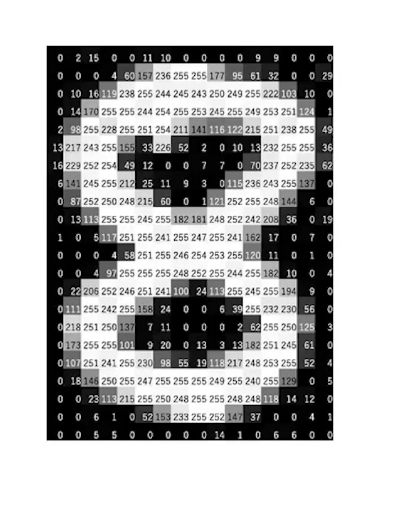
\includegraphics[width=0.4\textwidth]{graphics/eight-pixels.png}
\end{center}
\end{frame}

%\begin{frame}
%\frametitle{Convoluties}
%
%Een convolutie is een bewerking waarbij een klein venster (bv.\ $3\times 3$) verschoven wordt 
%over een groter beeld. 
%
%\vspace{0.5cm}
%
%De pixels die overlappen in het grote beeld en in het kleine venster worden twee aan twee met elkaar vermenigvuldigd 
%en daarna opgeteld. Dit is dan een nieuwe \lq\lq pixel\rq\rq\ in het uitvoerbeeld.
%
%\vspace{0.5cm}
%
%%Dit klinkt ingewikkeld, maar eigenlijk is het eenvoudig! Zie Excel-bestand \texttt{vijf.xlsx}.
%
%\end{frame}
%
%\begin{frame}
%\frametitle{Convolutie: Voorbeeld}
%
%\begin{center}
%	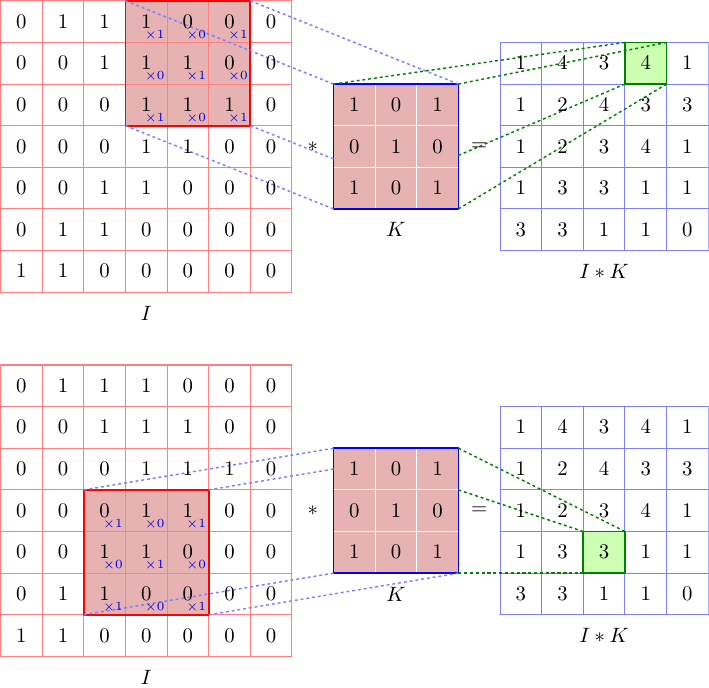
\includegraphics[width=0.5\textwidth]{graphics/conv-1}
%\end{center}
%
%\end{frame}
%
%\begin{frame}
%\frametitle{Convolutie: 3D-Animatie}
%Zie \url{https://animatedai.github.io/}.
%\end{frame}
%
%\begin{frame}
%\frametitle{Convolutie: Python Notebook}
%Ga zelf aan de slag met de notebook \texttt{TestConvoluties.ipynb} om 
%wat extra intu\"{\i}tie op te doen m.b.t.\ convoluties.
%\end{frame}
%
%
%\begin{frame}
%\frametitle{Convoluties: leren}
%
%\begin{itemize}
%\item Convoluties zijn niet nieuw en werden al gebruikt lang voor machine en deep learning populair waren.
%\item Traditioneel werden de convoluties \lq\lq handmatig\rq\rq\ bepaald om bepaalde zaken te detecteren
%(bv.\ horizonale of verticale randen).
%\item Binnen machine learning zijn de waarden in het venstertje \emph{parameters}\/ van het model 
%die worden bepaald (i.e.\ geleerd) door het algoritme. 
%(Dus net zoals de parametes $a$ en $b$ bij lineaire regressie.)
%\item In \'e\'en bepaalde laag zijn er typsich \emph{veel} \lq\lq venstertjes\rq\rq\ om te leren!
%\begin{itemize}
%	\item Het getransformeerde beeld krijgt dus altijd meer en meer lagen (evenveel als er venstertjes zijn).
%\end{itemize}
%
%\end{itemize}
%\end{frame}
%
%\begin{frame}
%\frametitle{Convolutionele NN: Details}
%\begin{itemize}
%\item Na het uitvoeren van de convolutie worden typisch de negatieve woorden gewoon op nul gezet 
%(en de andere blijven gewoon behouden).
%\begin{itemize}
%	\item De offici\"ele naam hiervoor is de \lq\lq Rectified Linear Unit\rq\rq\, typisch afgekort tot ReLu.
%\end{itemize}		
%\item Om het aantal parameters onder controle te houden worden de hoogte en breedte van het beeld 
%dan (typisch) gehalveerd m.b.v. een max pooling laag.
%\item Op het einde van een convolutioneel NN komen er typisch nog een aantal volledig geconnecteerde lagen, 
%met op het einde een laag die de verschillende klassen voorstellen.
%\end{itemize}
%\end{frame}



\begin{frame}
\frametitle{ImageNet Competitie}

\begin{itemize}
\item ImageNet bestaat uit een groot aantal afbeeldingen (meer dan 1.000.000) onderverdeeld in 1000 klassen.
\item Gebruikt als een prestigieuze competitie om \lq\lq computer vision\rq\rq\ mogelijkheden te evalueren.
\end{itemize}

\begin{center}
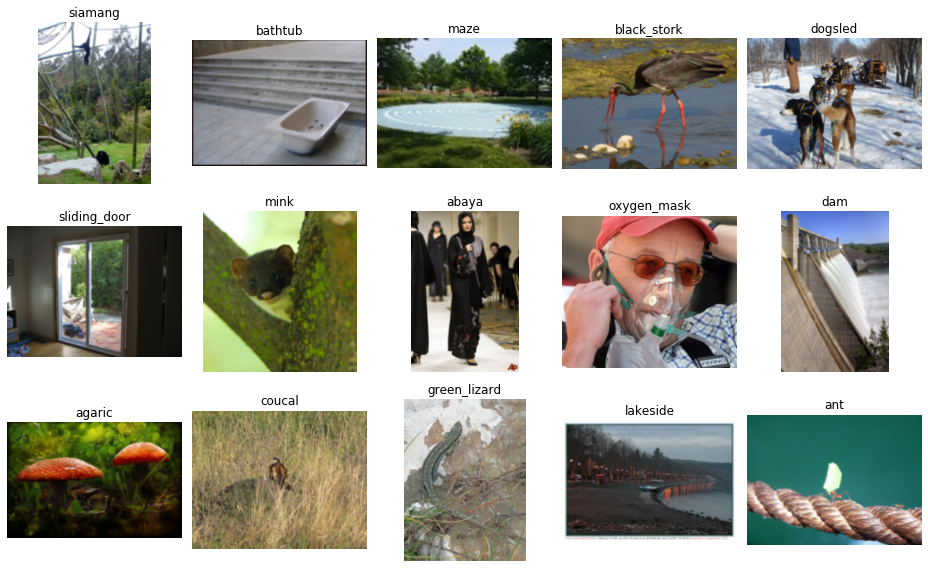
\includegraphics[width=0.50\textwidth]{graphics/imagenet-dogsled}
\end{center}

\end{frame}

\begin{frame}
\frametitle{AlexNet}

\begin{itemize}
	\item Alex Krizhevsky nam in 2012 samen met Ilya Sutskever en Geoffrey Hinton deel aan de ImageNet competitie met een convolutioneel neuraal netwerk.
	\item Hij won, en hoe! Zijn model had \lq\lq top five error rate\rq\rq\ van 16 procent, het model 
	op de tweede plaats haalde 26 procent.
\end{itemize}

\end{frame}

%\begin{frame}
%\frametitle{AlexNet: Architectuur}
%\vspace{-0.5cm}
%\begin{center}
%	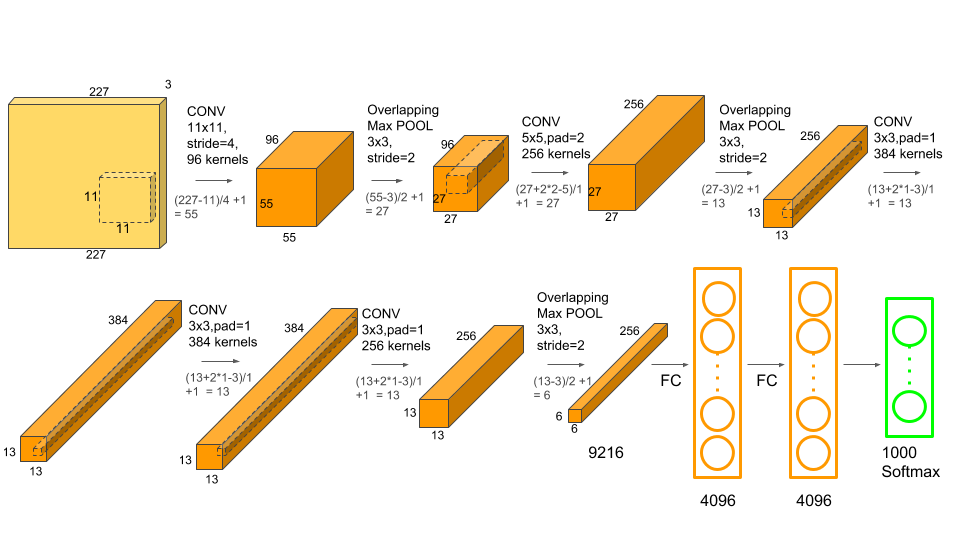
\includegraphics[width=0.80\textwidth]{graphics/alexnet-architecture}
%\end{center}
%\end{frame}
%
%\begin{frame}
%\frametitle{Algemene Architectuur NN}
%	
%\begin{block}{Architectuur Neuraal Netwerk}
%Een neuraal netwerk
%\begin{itemize}
%\item Bestaat uit een (groot) aantal lagen.
%\item Elke laag voert een relatief eenvoudige bewerking uit.
%\item Samen vormen de lagen een (ingewikkelde) wiskundige functie die invoer 
%op uitvoer afbeeldt.
%\end{itemize}
%\end{block}
%
%De parameters van het neuraal netwerk worden getraind met (een variant van) gradient descent
%om de \lq\lq optimale\rq\rq\ waarden van de parameters te bekomen.
%	
%
%\end{frame}


%
%\begin{frame}
%\frametitle{Tensorflow/Keras}
%
%
%\begin{itemize}
%	\item Tensorflow en Keras zijn softwarebibliotheken die het mogelijk maken om zeer krachtige 
%	Deep Learning modellen en applicaties te ontwikkelen op een zeer effici\"ente manier.
%	\item Op de volgende slide defini\"eren en trainen we AlexNet op \'e\'en enkele slide!
%	\begin{itemize}
%		\item In 2012 was dit baanbrekend onderzoek en nu beschikbaar voor iedereen.
%	\end{itemize}
%\end{itemize}
%\begin{center}
%
\includegraphics[width=0.5\textwidth]{graphics/tensorflow-keras}
%\end{center}
%\end{frame}

%\begin{frame}[fragile=singleslide]
%\frametitle{AlexNet in Keras}
%\begin{lstlisting}[language = Python , frame = trBL , firstnumber = 1 , escapeinside={(*@}{@*)}, basicstyle=\tiny \ttfamily]
%# Definieer model
%model=keras.models.Sequential([
%	keras.layers.Conv2D(filters=96, kernel_size=(11,11), strides=(4,4), activation='relu', padding='valid', input_shape=(227,227,3)),
%	keras.layers.MaxPool2D(kernel_size=(3,3), pool_size=(2,2), padding='valid'),
%	keras.layers.Conv2D(filters=256, kernel_size=(5,5), strides=(1,1), activation='relu', padding="same"),
%	keras.layers.MaxPool2D(kernel_size=(3,3), pool_size=(2,2), padding='valid'),
%	keras.layers.Conv2D(filters=384, kernel_size=(3,3), strides=(1,1), activation='relu', padding="same"),
%	keras.layers.Conv2D(filters=384, kernel_size=(3,3), strides=(1,1), activation='relu', padding="same"),
%	keras.layers.Conv2D(filters=256, kernel_size=(3,3), strides=(1,1), activation='relu', padding="same"),
%	keras.layers.MaxPool2D(kernel_size=(3,3), pool_size=(2,2), padding='valid'),
%	keras.layers.Flatten(),
%	keras.layers.Dense(4096,activation='relu'),
%	keras.layers.Dense(4096,activation='relu'),
%	keras.layers.Dense(1000,activation='softmax')  
%])
%# Specifieer opties om te trainen
%model.compile(
%	loss='sparse_categorical_crossentropy',
%	optimizer=tf.optimizers.SGD(lr=0.001),
%	metrics=['accuracy']    
%)
%# Train het model
%history=model.fit(train_ds, epochs=50, validation_data=test_ds)
%\end{lstlisting}
%\end{frame}

%\begin{frame}
%\frametitle{Transfer Learning}
%
%Het kan nog gemakkelijker dan het zelf implementeren van AlexNet.
%
%\begin{itemize}
%	\item Het blijkt dat de eerste lagen van een convolutioneel neuraal netwerk (zoals AlexNet) dingen leren 
%	die nuttig zijn voor \emph{alle soorten van classificatietaken} voor beelden.
%	\begin{itemize}
%		\item De eerste lagen herkennen zaken als randen, hoeken, cirkels, etc.
%		\item Hogere lagen combineren deze in zaken als 'gezicht': (twee cirkels op bepaalde plaats, twee horizontale randen (lippen), )
%	\end{itemize}
%	\item Hoe verder men komt in de lagen, hoe meer specifiek die zijn voor de taak waarvoor het netwerk getraind is.
%\end{itemize}
%\end{frame}

%\begin{frame}	
%\frametitle{Transfer Learning Visueel}
%
%\begin{center}
%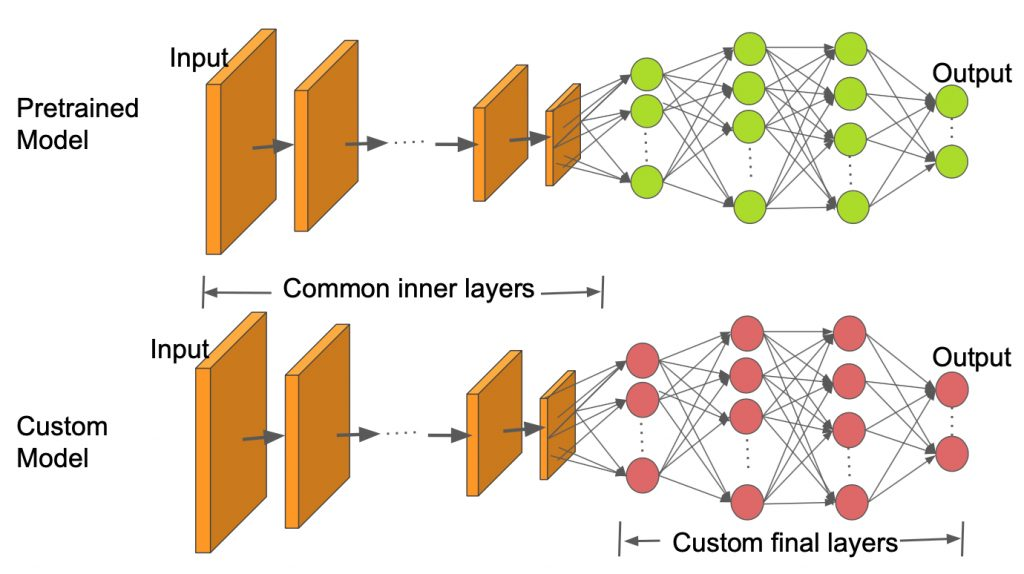
\includegraphics[width=0.8\textwidth]{graphics/transfer-learning}
%\end{center}
%
%\end{frame}

%\begin{frame}
%\frametitle{Notebook Transfer Learning}
%Open de notebook \texttt{WorkshopML\_TransferLearning} om transfer learning in actie te zien 
%om honden en katten van elkaar te kunnen onderscheiden.
%\end{frame}



%\begin{frame}
%\frametitle{Trainen van een ML model zonder code}
%\begin{itemize}
%\item  We gebruiken de \texttt{AutoTrain}-feature van Hugging Face om een hond-vs-kat classificatiemodel
%te maken.
%\item Dit classificatiemodel kan dan aangesproken worden over het Internet.
%\item Merk op: dit model werd (hoogstwaarschijnlijk) getraind via \textbf{transfer learning}.
%\end{itemize}
%\end{frame}


\begin{frame}
\frametitle{Trainen van een ML model zonder code}
\begin{itemize}
\item  We gebruiken Google Teachable Machine om een classificatiemodel aan te maken.
\item Dit classificatiemodel kan dan aangesproken worden in een Python notebook.
\item Merk op: dit model werd (hoogstwaarschijnlijk) getraind via \textbf{transfer learning}.
\end{itemize}
\end{frame}


\begin{frame}
\frametitle{Transfer Learning}
\begin{itemize}
\item Bij \textbf{transfer learning} wordt een bestaand model hergebruikt voor een gelijkaardige (maar verschillende taak).
\item Bv.\ voor de classificatie van honden vs.\ katten kunnen we gebruikmaken van een netwerk 
dat werd getraind op ImageNet, en dat dus 1000 verschillende  klassen kan herkennen.
\begin{itemize}
	\item De laatste laag van dit model bestaat uit 1000 neuronen.
\end{itemize}
\item We vervangen de laatste (en meest specifieke) laag door een nieuwe laag (met twee neuronen)
 die honden van katten kan onderscheiden.
\end{itemize}
\end{frame}


%\begin{frame}
%\frametitle{Demo AutoTrain Hugging Face}
%\begin{itemize}
%\item Maak een (gratis) account op Hugging Face: \url{https://huggingface.co/}
%\item Bedenk twee (of meer) categorie\"en die je van elkaar wil kunnen onderscheiden.
%\item  Gebruik een zoekmachine om een aantal afbeeldingen van 
%elke categorie te verzamelen: minstens 10 afbeeldingen in elke categorie.
%\item Volg stappenplan bij de AutoTrain feature.
%\item \lq\lq Deploy\rq\rq\ je model en roep het aan vanuit Python (bv.\ Google Colab) om voorspellingen 
%te krijgen.
%\end{itemize}
%\end{frame}


\begin{frame}
\frametitle{Maak het hond/wolf model beter}

\begin{enumerate}
\item Zoek extra trainingsafbeeldingen om het hond/wolf model beter te maken.
\item Kan je het model aan de praat krijgen in een Python notebook?
\end{enumerate}

\end{frame}


\begin{frame}
\frametitle{Maak je eigen model!}

\begin{enumerate}
\item Bedenk een leuk classificatieprobleem op basis van afbeeldingen.
\item Verzamel op het internet afbeeldingen van de verschillende klassen.
\item Train een model met Google Teachable Machine (\url{https://teachablemachine.withgoogle.com/})
\item Sla het model op met Tensorflow.
\item Gebruik Google Colab om m.b.v.\ code je model aan te roepen op (nieuwe) afbeeldingen.
\end{enumerate}
\end{frame}

%\section{Generatieve Modellen}

%\begin{frame}
%\frametitle{Beeldgeneratie met Stable Diffusion}
%
%\end{frame}

\begin{frame}
\frametitle{Workshop Conclusie}
\begin{itemize}
\item Wees niet ontgoocheld als je vandaag niet alles hebt begrepen:
\begin{itemize}
	\item Van basis Machine Learning t.e.m.\ Transfer Learning zijn in de opleiding Toegepaste Informatica \textbf{twee} vakken in het tweede en derde jaar!
\end{itemize}
\item Een diepgaande kennis van de wiskunde en de algoritmen is niet nodig om succesvol te zijn in Machine Learning.
\begin{itemize}
	\item Het is \emph{wel}\/ nodig om logisch te kunnen nadenken!
	\item Het helpt om te snappen wat er gebeurt in de modellen op het moment dat het fout loopt, zodat je effici\"ent kan 
	debuggen.
\end{itemize}
\item In de opleiding Toegepaste Informatica leer je niet alleen over wat je vandaag hebt gezien maar ook 
wat er nodig is om je model \lq\lq in productie\rq\rq\ te gebruiken.
\begin{itemize}
	\item Dit uiteraard naast de basisvaardigheden die je nodig hebt\\ om aan de slag te gaan
	 als \textbf{all-round informaticus}.
\end{itemize}
\end{itemize}
\end{frame}



\end{document}